
\begin{figure}
    \centering
    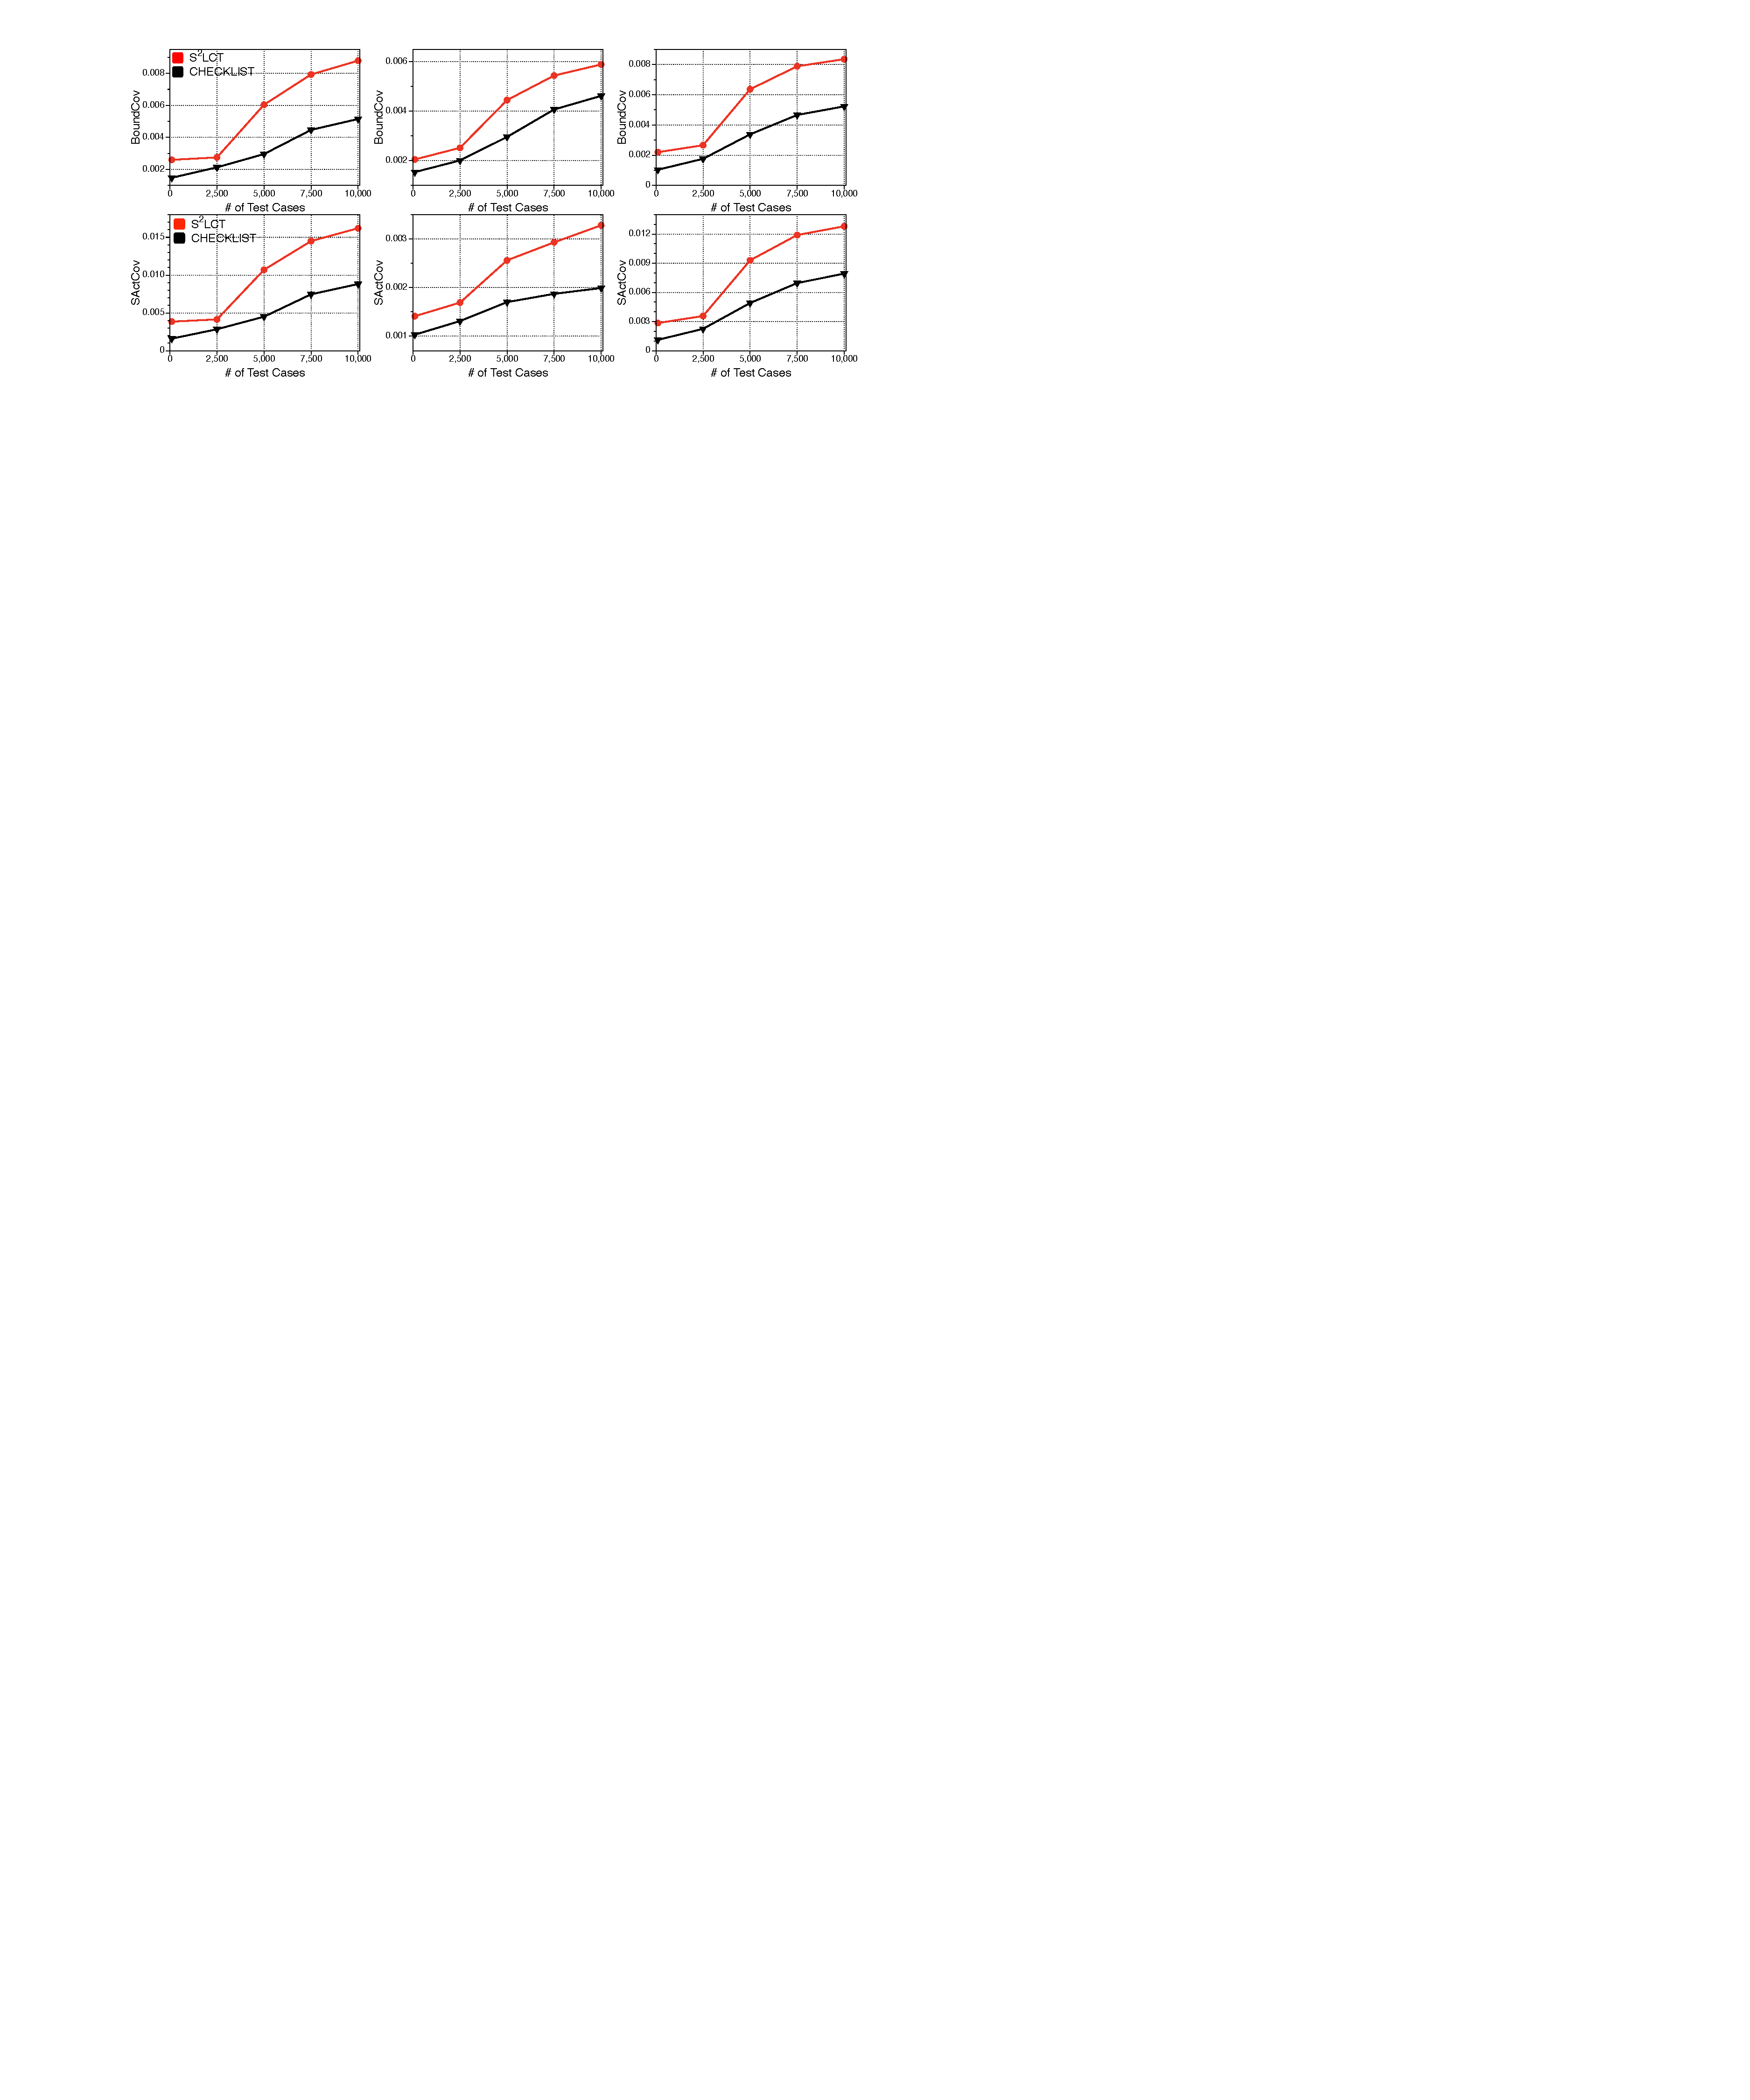
\includegraphics[width=0.5\textwidth]{figs/covergae.pdf}
    \caption{The coverage results of the generated test
      samples. \sw{Make the figures larger.}}
    \label{fig:coverage}
\end{figure}


Fig. \ref{fig:coverage} shows the coverage results of the generated
test samples, where the red line represents \tool and the black line
represents \Cklst.  Each column in Fig. \ref{fig:coverage} represent
the results for one NLP model, the first row is the \textit{BoundCov}
results and the second row is the \textit{SActCov} results.  From the
results, we make two observations observations. First, for \emph{all}
experimental settings (\eg NLP model, coverage metric), \tool achieves
high coverage than \Cklst. Recall that a higher coverage implies the
test case in the test suite is more diverse and rarely to have a
statistical distribution similar to the model training data. As a
result, a test suite with greater coverage complements the model
training data distribution (\ie hold-out testing data) better.  The
experimental results confirm that \tool can generate more diverse test
cases to complement the hold-out testing data for testing NLP models.
\sw{What does the growth trend in each figure indicate?} \sw{Does the
  absolute numbers or relative difference of the two lines on y axis
  mean anything concrete? E.g., how significant is the improvement in
  diversity?}

Another interesting finding is that for each NLP model, there is no
fixed relationship between \textit{BoundCov} and \textit{SActCov}. In
other words, while a test suite may produce higher \textit{BoundCov}
for some models, the same test suite may get higher \textit{SActCov}
for other NLP models.  Recall that \textit{BoundCov} measures both the
upper and lower corner neurons and \textit{SActCov} measures only the
upper corner neurons.  Such observation implies that the upper and
lower corner neurons are distributed unevenly, and measuring only one
of them is not enough.
